% Mercury: the HF modem of HERMES -- recent developments (October 2026)
% Build: make  (pdflatex twice; needs texlive with beamer, metropolis, FiraSans, pgfplots)
% Copyright (C) 2026 Rhizomatica
% SPDX-License-Identifier: CC-BY-SA-4.0
\documentclass[aspectratio=169,10pt]{beamer}

\usetheme[progressbar=frametitle,numbering=fraction,sectionpage=progressbar,block=fill]{metropolis}
\usepackage[sfdefault,lining]{FiraSans}
\usepackage[T1]{fontenc}
\usepackage[utf8]{inputenc}
\usepackage{booktabs,array,colortbl,multirow}
\usepackage{tikz,pgfplots}
\usetikzlibrary{arrows.meta,positioning,calc,shapes.geometric,fit,backgrounds}
\pgfplotsset{compat=1.18}
\usepackage{fontawesome5}

% ---- the HERMES palette (hermes.radio) ------------------------------------
\definecolor{hcream}{HTML}{FFF6C0}
\definecolor{hcreamdk}{HTML}{F6E9A4}
\definecolor{hgreen}{HTML}{96B863}
\definecolor{hdkgreen}{HTML}{5E743E}
\definecolor{horange}{HTML}{FF6600}
\definecolor{hblack}{HTML}{1E1D1D}
\definecolor{hmauve}{HTML}{CD97BD}
\definecolor{hdkmauve}{HTML}{A17895}

\setbeamercolor{normal text}{fg=hblack,bg=hcream}
\setbeamercolor{background canvas}{bg=hcream}
\setbeamercolor{frametitle}{fg=white,bg=hdkgreen}
\setbeamercolor{progress bar}{fg=horange,bg=hgreen}
\setbeamercolor{title separator}{fg=horange}
\setbeamercolor{alerted text}{fg=horange}
\setbeamercolor{example text}{fg=hdkgreen}
\setbeamercolor{block title}{fg=white,bg=hdkgreen}
\setbeamercolor{block body}{fg=hblack,bg=hcreamdk}
\setbeamercolor{block title alerted}{fg=white,bg=horange}
\setbeamercolor{block body alerted}{fg=hblack,bg=hcreamdk}
\setbeamercolor{block title example}{fg=white,bg=hdkmauve}
\setbeamercolor{block body example}{fg=hblack,bg=hcreamdk}
\setbeamercolor{itemize item}{fg=hdkgreen}
\setbeamercolor{itemize subitem}{fg=horange}
\setbeamercolor{page number in head/foot}{fg=hdkgreen}
\setbeamerfont{frametitle}{series=\bfseries,size=\large}
\setbeamerfont{section title}{series=\bfseries}
\setbeamertemplate{itemize item}{\color{hdkgreen}\scriptsize$\blacktriangleright$}
\setbeamertemplate{itemize subitem}{\color{horange}\tiny$\bullet$}
\makeatletter
\setlength{\metropolis@titleseparator@linewidth}{1.5pt}
\setlength{\metropolis@progressonsectionpage@linewidth}{2pt}
\makeatother

% Section pages: the foliage band above the title.
\setbeamertemplate{section page}{%
  \centering
  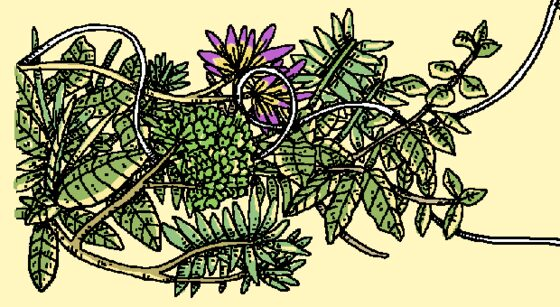
\includegraphics[height=0.32\textheight]{img/foliage-band.jpg}\par\vspace{1.2em}
  {\usebeamerfont{section title}\usebeamercolor[fg]{normal text}\LARGE\MakeUppercase{\insertsectionhead}}\par
  \vspace{0.6em}
  {\color{horange}\rule{0.35\textwidth}{2pt}}\par
}

\newcommand{\ours}{\cellcolor{hgreen!35}}
% Sources sit on the bottom edge, outside the text area, so they take no room.
\newcommand{\src}[1]{\begin{tikzpicture}[remember picture,overlay]
  \node[anchor=south west,inner sep=0,font=\tiny,text=hdkmauve] at ($(current page.south west)+(0.42cm,0.2cm)$) {#1};
\end{tikzpicture}}
\newcommand{\hl}[1]{{\color{horange}\bfseries #1}}

\title{Mercury}
\subtitle{The HF modem and ARQ of HERMES --- what we built in 2026}
\author{Rhizomatica}
\date{October 2026}

\begin{document}

% ---- title ------------------------------------------------------------------
\begin{frame}[plain]
  \begin{tikzpicture}[remember picture,overlay]
    \fill[hcream] (current page.south west) rectangle (current page.north east);
    \node[anchor=north east,inner sep=0] at (current page.north east)
      {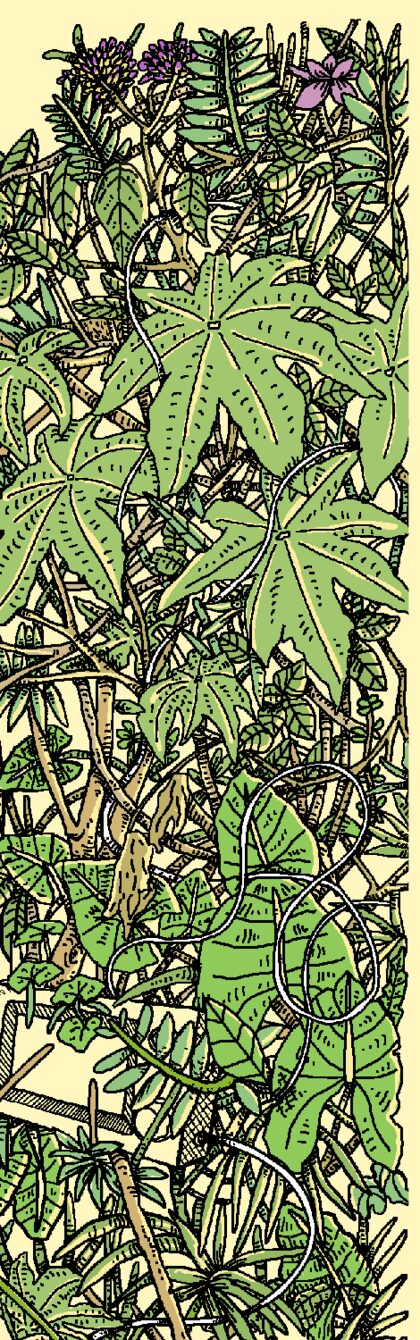
\includegraphics[height=\paperheight]{img/foliage-strip.jpg}};
    \node[anchor=north west,inner sep=0] at ($(current page.north west)+(1.0cm,-0.9cm)$)
      {
\includegraphics[height=2.6cm]{img/hermes-logo.png}};
    \node[anchor=north west,text width=10cm,inner sep=0] at ($(current page.north west)+(1.0cm,-4.0cm)$) {%
      {\fontsize{38}{40}\selectfont\bfseries MERCURY}\par\vspace{0.25em}
      {\color{horange}\rule{3.5cm}{2.5pt}}\par\vspace{0.6em}
      {\large The HF modem and ARQ of HERMES}\par\vspace{0.2em}
      {\normalsize New modes, MFSK, a new ARQ, formal proofs\\ and a standard-compliant test framework}\par\vspace{1.2em}
      {\small\color{hdkgreen}\bfseries Rhizomatica \quad\textbullet\quad October 2026}\par
      {\scriptsize\color{hdkmauve}github.com/Rhizomatica/mercury \quad\textbullet\quad hermes.radio}};
  \end{tikzpicture}
\end{frame}

\begin{frame}{Outline}
  \begin{columns}[T]
    \column{0.5\textwidth}
    \begin{enumerate}
      \item Mercury in HERMES
      \item The modes: a ladder of our own
      \item MFSK: the fringe of the link
      \item The carousel: a new ARQ
    \end{enumerate}
    \column{0.5\textwidth}
    \begin{enumerate}\setcounter{enumi}{4}
      \item Formal methods: TLA+ and TLAPS
      \item Testing, and a standard channel
      \item Integration and platforms
      \item What comes next
    \end{enumerate}
  \end{columns}
\end{frame}

% =============================================================================
\section{Mercury in HERMES}

\begin{frame}{What Mercury is}
  \small
  \begin{columns}[T]
    \column{0.56\textwidth}
    \begin{itemize}
      \item The HF software modem of \textbf{HERMES}: it turns an SSB radio into a data link for email, files and messages
      \item Hands the application a \textbf{TCP connection}: a VARA-compatible TNC (control 8300, data 8301), KISS and broadcast on 8100
      \item A clean \textbf{rewrite in C} (v2, since March 2026); the C++ v1 lives on as \texttt{mercuryv1}
      \item \textbf{Free software}: GPL-3.0-or-later; vendored codec2 subset LGPL-2.1
      \item Built by Rhizomatica for communities beyond the Internet, first in the Amazon rainforest
    \end{itemize}
    \column{0.42\textwidth}
    \begin{tikzpicture}[node distance=0.32cm,
        box/.style={draw=hdkgreen,fill=white,rounded corners=2pt,minimum width=4.6cm,minimum height=0.62cm,font=\small,line width=0.8pt},
        acc/.style={box,fill=hgreen!45,font=\small\bfseries}]
      \node[box] (app) {UUCP \,·\, NNCP \,·\, JNOS \,·\, Reticulum};
      \node[box,below=of app] (tnc) {TNC \,/\, KISS \,/\, WebSocket UI};
      \node[acc,below=of tnc] (arq) {Carousel ARQ \,·\, broadcast};
      \node[acc,below=of arq] (mod) {Modem: OFDM ladder + MFSK};
      \node[box,below=of mod] (aud) {Audio + PTT \,(ALSA, RTP, CoreAudio, ...)};
      \node[box,below=of aud,fill=hcreamdk] (rad) {SSB transceiver \faBroadcastTower};
      \foreach \a/\b in {app/tnc,tnc/arq,arq/mod,mod/aud,aud/rad}
        \draw[-{Latex[length=2mm]},hdkgreen,line width=0.8pt] (\a) -- (\b);
    \end{tikzpicture}
  \end{columns}
\end{frame}

\begin{frame}{2026 in numbers}
  \begin{columns}[c]
    \column{0.5\textwidth}
    \centering
    \begin{tikzpicture}
      \foreach \v/\l/\y in {1109/{commits on trunk since the C rewrite (2026-03-05)}/0,
                            496/{commits since 1 September}/-1.35,
                            5/{releases since September (1.9.15 \textrightarrow{} 1.9.19)}/-2.7}{
        \node[anchor=east,font=\fontsize{30}{30}\selectfont\bfseries,text=horange] at (0,\y) {\v};
        \node[anchor=west,text width=4.6cm,font=\small] at (0.25,\y) {\l};
      }
    \end{tikzpicture}
    \column{0.5\textwidth}
    \begin{block}{Platforms}
      Linux (amd64, arm64, armhf, i386), Raspberry Pi 4/5, Windows (signed), macOS (universal, notarised); \textbf{iOS and Android coming soon}
    \end{block}
    \begin{block}{Releases}
      \textbf{1.9.18} (12 Oct): the carousel data plane\\
      \textbf{1.9.19} (13 Oct): MFSK centred on 1500 Hz, protocol v2, JNOS 2.0
    \end{block}
  \end{columns}
  \src{Source: git history of \texttt{mercuryv2}; docs/RELEASE-1.9.18.md, docs/RELEASE-1.9.19.md}
\end{frame}

\begin{frame}{1.9.18 against 1.9.17: the same 2 KB, one way}
  \begin{columns}[c]
    \column{0.6\textwidth}
    \begin{tikzpicture}
      \begin{axis}[ybar,width=8.6cm,height=5.4cm,bar width=13pt,
          ymin=0,ymax=560,ylabel={seconds (lower is better)},
          symbolic x coords={+10 dB,0 dB,$-7$ dB,$-10$ dB},xtick=data,
          enlarge x limits=0.18,legend style={at={(0.02,0.98)},anchor=north west,fill=hcream,draw=none,font=\small},
          axis background/.style={fill=hcream},axis line style={hblack},tick label style={font=\small},
          nodes near coords,every node near coord/.append style={font=\scriptsize},
          ymajorgrids,grid style={hcreamdk}]
        \addplot[fill=hmauve,draw=hdkmauve] coordinates {(+10 dB,76) (0 dB,268)};
        \addplot[fill=hgreen,draw=hdkgreen] coordinates {(+10 dB,34) (0 dB,146) ($-7$ dB,458) ($-10$ dB,417)};
        \legend{1.9.17,1.9.18}
        \node[font=\scriptsize\bfseries,text=hdkmauve,rotate=90,anchor=west,xshift=-7pt] at (axis cs:$-7$ dB,15) {1.9.17 failed};
        \node[font=\scriptsize\bfseries,text=hdkmauve,rotate=90,anchor=west,xshift=-7pt] at (axis cs:$-10$ dB,15) {1.9.17 failed};
      \end{axis}
    \end{tikzpicture}
    \column{0.38\textwidth}
    \begin{itemize}
      \item Two real daemons through codec2 \texttt{ch}, 2074 bytes
      \item \hl{2$\times$ faster} on a good link
      \item Links down to \hl{$-10$ dB} SNR now complete
      \item On air, 8 KB each way: 485/509 s \textrightarrow{} \textbf{312/238 s}
      \item At 3 \% power, 2 KB: 1310/1266 s \textrightarrow{} \textbf{832/755 s}
    \end{itemize}
  \end{columns}
  \src{Source: docs/RELEASE-1.9.18.md}
\end{frame}

% =============================================================================
\section{The modes: a ladder of our own}

\begin{frame}{The mode table}
  \centering\footnotesize\setlength{\tabcolsep}{4.5pt}
  \begin{tabular}{@{}l l r r r l l@{}}
    \toprule
    \textbf{Mode} & \textbf{Origin} & \textbf{BW, Hz} & \textbf{Payload, B} & \textbf{bit/s} & \textbf{FEC (n,k)} & \textbf{Role} \\
    \midrule
    \ours MFSK     & \ours Mercury           & \ours 1000 & \ours 98   & \ours $\sim$60 & \ours LDPC (1600,800)   & \ours rung 0 (floor) \\
    \ours DATAC15  & \ours Mercury           & \ours 200  & \ours 30   & \ours 68       & \ours (768,256)          & \ours rung 1 \\
    DATAC4         & codec2                  & 250        & 54         & 87             & (1472,448)               & rung 2 \\
    DATAC3         & codec2                  & 500        & 126        & 321            & (2048,1024)              & rung 3 (BW500 top) \\
    DATAC1         & codec2                  & 1700       & 510        & 980            & (8192,4096)              & rung 4 \\
    \ours DATAC17  & \ours Mercury           & \ours 2100 & \ours 1180 & \ours 1410     & \ours (15936,9456)       & \ours rung 5 \\
    QAM16C2        & codec2                  & 2100       & 1213       & 3100           & (16200,9720)             & rung 6 \\
    \midrule
    \ours DATAC16  & \ours Mercury           & \ours 200  & \ours 14   & \ours 42       & \ours (640,128)          & \ours ARQ control \\
    DATAC0/13/14   & codec2                  & 200--500   & 3--14      & 58--291        & ---                      & broadcast, tests \\
    \bottomrule
  \end{tabular}
  \par\medskip
  {\small\colorbox{hgreen!35}{\strut\, green \,} = designed by us: three of the seven rungs, and the control mode}
  \src{Source: docs/MODES.md}
\end{frame}

\begin{frame}{The ladder: seven rungs, 60 to 3100 bit/s}
  \centering
  \begin{tikzpicture}[x=1.75cm,y=0.62cm]
    \foreach \i/\m/\r/\s/\c in {0/MFSK/60/floor/hgreen,1/DATAC15/68/$\geq -3$/hgreen,2/DATAC4/87/probe/hcreamdk,
                                3/DATAC3/321/$\geq +1$/hcreamdk,4/DATAC1/980/$\geq +8$/hcreamdk,
                                5/DATAC17/1410/$\geq +12$/hgreen,6/QAM16C2/3100/$\geq +18$/hcreamdk}{
      \fill[\c,draw=hdkgreen,line width=0.7pt,rounded corners=1.5pt] (\i,0) rectangle ++(0.92,0.85*\i+1.7);
      \node[font=\scriptsize\bfseries,rotate=90,anchor=west] at (\i+0.46,0.15) {\m};
      \node[font=\scriptsize,anchor=south] at (\i+0.46,0.85*\i+1.7) {\r\ bit/s};
      \node[font=\scriptsize,text=hdkmauve,anchor=north] at (\i+0.46,-0.15) {\s};
    }
    \draw[-{Latex[length=3mm]},horange,line width=1.5pt] (-0.2,-1.6) -- (7.0,-1.6) node[right,font=\small\color{hblack}] {SNR};
    \node[anchor=west,font=\scriptsize,text=hdkmauve] at (-0.25,-2.2) {start rung chosen by the SNR the caller measured (dB); then link adaptation by measured goodput};
    \draw[hdkgreen,dashed,line width=0.8pt] (3.96,-0.6) -- (3.96,7.3) node[above,font=\scriptsize\color{hdkgreen}] {BW500 cap};
  \end{tikzpicture}
  \src{Source: datalink\_arq/carousel.c (car\_start\_level), docs/CAROUSEL-SPEC.md \S 15}
\end{frame}

\begin{frame}{Our OFDM modes}
  \small
  \begin{columns}[T]
    \column{0.5\textwidth}
    \begin{block}{Robust: DATAC15 and DATAC16}
      \begin{itemize}
        \item Rate-1/3 LDPC (\texttt{H\_256\_768\_22}), 200 Hz
        \item DATAC15: 30 bytes, 3 carriers, the first OFDM rung
        \item DATAC16: 14 bytes, calls, polls and ACKs
        \item 70/100 frames at $-7$ dB on MPP fading
      \end{itemize}
    \end{block}
    \column{0.5\textwidth}
    \begin{block}{Fast: DATAC17, on codec2's QAM16C2 code}
      \begin{itemize}
        \item 2.1 kHz, about 1.2 KB a frame
        \item codec2's QAM16C2: 16-QAM, (16200,9720), 3100 bit/s
        \item DATAC17: QPSK on that codeword, 1410 bit/s
        \item DATAC17 97/100 at +10 dB (MPP)
      \end{itemize}
    \end{block}
  \end{columns}
  \smallskip
  \begin{exampleblock}{Making the ladder honest}
    \footnotesize Per-mode \textbf{SNR calibration} (QAM16C2 read 9 dB low); a 16-QAM estimator above 12 dB;
    the \textbf{TX filter} no longer cuts our outer carriers (6.5 dB); \textbf{FFT-correlation} acquisition, 2.2$\times$ cheaper
  \end{exampleblock}
  \src{Source: docs/MODES.md, docs/OTA-PHASE-A-SNR-CALIB.md; PRs \#163, \#337, \#350}
\end{frame}

% =============================================================================
\section{MFSK: the fringe of the link}

\begin{frame}{MFSK: a non-coherent floor under the OFDM ladder}
  \begin{columns}[T]
    \column{0.52\textwidth}
    \begin{itemize}
      \item Mercury's own modem: \textbf{32-FSK on OFDM subcarriers}, non-coherent
      \item 8 kHz, Nfft 256: tones 31.25 Hz apart, 40 ms symbols (25 baud)
      \item Centred on \textbf{1500 Hz} since 1.9.19: tones 1015.6--1984.4 Hz
      \item Preamble \emph{and} postamble: a burst is found from either end
      \item LDPC N = 1600; five rates ported, \textbf{rate 1/2 ships} (98-byte frames, 13.5 s)
      \item Lowering the rate to 1/16 buys only 2.1 dB: the floor is set by sync, not by the code
    \end{itemize}
    \column{0.45\textwidth}
    \begin{tikzpicture}
      \begin{axis}[width=6.6cm,height=5.2cm,xmin=900,xmax=2100,ymin=0,ymax=1.35,
          xlabel={Hz},ytick=\empty,axis background/.style={fill=hcream},
          tick label style={font=\scriptsize},label style={font=\scriptsize},axis lines=left]
        \foreach \k in {0,...,31}{
          \edef\temp{\noexpand\addplot[hgreen,line width=1.4pt] coordinates {(1015.625+31.25*\k,0) (1015.625+31.25*\k,0.55)};}
          \temp
        }
        \addplot[horange,line width=2.2pt] coordinates {(1015.625+31.25*19,0) (1015.625+31.25*19,1.1)};
        \node[font=\scriptsize,text=horange,anchor=south] at (axis cs:1609,1.12) {one tone a symbol: 5 bits};
      \end{axis}
    \end{tikzpicture}
    \par\small\centering The 32 tones, 1015.6--1984.4 Hz
  \end{columns}
  \src{Source: docs/MFSK-PORT.md, modem/modem\_mfsk.c, docs/RELEASE-1.9.19.md}
\end{frame}

\begin{frame}{The floor was a threshold, not the code}
  \begin{columns}[c]
    \column{0.5\textwidth}
    \begin{itemize}
      \item All five code rates gave \textbf{identical} frame error rates: the decoder never saw the hard frames
      \item The sync accept gate was 0.5, which demands SNR per symbol $\geq$ 0 dB
      \item At \textbf{0.08}, with false anchors released:
      \begin{itemize}
        \item AWGN 50 \% point: $-0.6$ \textrightarrow{} \hl{$-11.2$ dB}
        \item Watterson 2 ms / 1 Hz: $+5.0$ \textrightarrow{} \hl{$-3.7$ dB}
      \end{itemize}
      \item Dual-ended acquisition is worth about 2 dB; interleaving the codeword 19 \% more fringe throughput
    \end{itemize}
    \column{0.48\textwidth}
    \begin{tikzpicture}
      \begin{axis}[xbar,width=6.6cm,height=5.0cm,bar width=10pt,xmin=-14,xmax=8,
          symbolic y coords={Watterson,AWGN},ytick=data,
          xlabel={SNR3k for 50 \% frames, dB},legend style={at={(0.5,1.03)},anchor=south,legend columns=2,font=\scriptsize,fill=hcream,draw=none},enlarge y limits=0.45,
          axis background/.style={fill=hcream},tick label style={font=\scriptsize},label style={font=\scriptsize},
          nodes near coords,every node near coord/.append style={font=\scriptsize},xmajorgrids,grid style={hcreamdk}]
        \addplot[fill=hmauve,draw=hdkmauve] coordinates {(5.0,Watterson) (-0.6,AWGN)};
        \addplot[fill=hgreen,draw=hdkgreen] coordinates {(-3.7,Watterson) (-11.2,AWGN)};
        \legend{gate 0.5,gate 0.08}
      \end{axis}
    \end{tikzpicture}
  \end{columns}
  \src{Source: docs/MFSK-PORT.md}
\end{frame}

\begin{frame}{Pattern ACKs: 0.64 seconds of air}
  \begin{columns}[T]
    \column{0.55\textwidth}
    \begin{itemize}
      \item An acknowledgement as a \textbf{Welch-Costas pattern}: 16 MFSK symbols, \textbf{0.64 s}
      \item 5.8$\times$ less airtime than a 3.74 s DATAC16 frame
      \item Detected every time down to about $-9$ dB on fading and $-22$ dB on AWGN
      \item \textbf{0 false alarms} in 30 trials down to $-26$ dB; 0 in 2 h of noise after the half-subcarrier search
      \item Frequency search over $\pm$78 Hz: an IC-7100 and an sBitx went from 0/5 to 17/17 patterns on air
    \end{itemize}
    \column{0.42\textwidth}
    \begin{tikzpicture}[x=0.22cm,y=0.13cm]
      \fill[hcreamdk] (0,0) rectangle (16,32);
      \foreach \t/\f in {0/3,1/7,2/15,3/30,4/27,5/21,6/9,7/18,8/5,9/11,10/23,11/14,12/28,13/24,14/16,15/1}{
        \fill[horange] (\t+0.1,\f) rectangle ++(0.8,1);
      }
      \draw[hdkgreen,line width=0.6pt] (0,0) rectangle (16,32);
      \node[font=\scriptsize,anchor=north] at (8,-0.6) {16 symbols = 0.64 s};
      \node[font=\scriptsize,rotate=90,anchor=south] at (-0.6,16) {32 tones};
    \end{tikzpicture}
    \par\smallskip\centering{\scriptsize (illustrative layout: one tone per symbol, no repeats)}
  \end{columns}
  \src{Source: docs/MFSK-PORT.md, README.md; PRs \#160, \#299}
\end{frame}

\begin{frame}{Sensitivity: MFSK against our best OFDM}
  \begin{columns}[c]
    \column{0.62\textwidth}
    \begin{tikzpicture}
      \begin{axis}[xbar,width=8.8cm,height=5.6cm,bar width=7pt,xmin=-16.5,xmax=5,
          symbolic y coords={DATAC3,DATAC4,DATAC15,MFSK floor,MFSK 500 Hz},ytick=data,
          xlabel={SNR3k for 90 \% delivery, dB (equal peak power)},
          legend style={at={(0.5,1.02)},anchor=south,legend columns=2,font=\scriptsize,fill=hcream,draw=none},
          axis background/.style={fill=hcream},tick label style={font=\scriptsize},label style={font=\scriptsize},
          nodes near coords,every node near coord/.append style={font=\tiny},xmajorgrids,grid style={hcreamdk},
          enlarge y limits=0.14]
        \addplot[fill=hgreen,draw=hdkgreen] coordinates {(0.2,DATAC3) (-4.3,DATAC4) (-6.1,DATAC15) (-11.1,MFSK floor) (-14.1,MFSK 500 Hz)};
        \addplot[fill=hmauve,draw=hdkmauve] coordinates {(2.3,DATAC15) (-6.8,MFSK floor) (-10.4,MFSK 500 Hz)};
        \legend{AWGN,moderate fading}
      \end{axis}
    \end{tikzpicture}
    \column{0.36\textwidth}
    \begin{itemize}
      \item MFSK holds \hl{5 to 9 dB} below DATAC15
      \item Against modem73's coherent RFDM modes: 2.7 dB better per bit on AWGN, a tie under fading
      \item On air: 1 KB over UUCP at \textbf{2 \% power} in 533 s
    \end{itemize}
  \end{columns}
  \src{Sim, 100 trials a point, Watterson model, 2026-10-15 (PR \#390); docs/MFSK-PORT.md; docs/RELEASE-1.9.19.md}
\end{frame}

\begin{frame}{In review: a 500 Hz MFSK, and a receiver that tracks the clock}
  \begin{columns}[T]
    \column{0.5\textwidth}
    \begin{block}{Mode 103 for 500 Hz filters (PR \#390)}
      \begin{itemize}
        \item The 1 kHz MFSK never decodes behind a 500 Hz CW filter
        \item 32 tones 15.625 Hz apart, 80 ms symbols, 26 s bursts
        \item 90 \%: \textbf{$-14.1$ dB} AWGN, $-10.4$ dB moderate, behind the filter too
        \item On air at the bench: $-14.2$ dB (sim $-14.1$)
      \end{itemize}
    \end{block}
    \column{0.5\textwidth}
    \begin{block}{Three receiver fixes, all modes}
      \begin{itemize}
        \item Dial offset to an eighth of a subcarrier
        \item Pattern search in half-subcarrier steps (removes a 3--4 dB loss)
        \item LLR noise from the tones' own bins
        \item Payload read at a \textbf{searched sample-clock ratio}: decodes from 0.98 to 1.02 (was $\pm$0.2 \%)
        \item Carrier offset as a top-level status field
      \end{itemize}
    \end{block}
  \end{columns}
  \src{Source: PR \#390 (draft), measurements 2026-10-15/16}
\end{frame}

% =============================================================================
\section{The carousel: a new ARQ}

\begin{frame}{Why a new ARQ}
  \begin{columns}[T]
    \column{0.5\textwidth}
    \begin{alertblock}{The old plane: SNR-driven stop-and-wait}
      \begin{itemize}
        \item One frame, one ACK, one turnaround
        \item Rungs chosen from SNR estimates that were wrong per mode
        \item Lost ACKs on the weak reverse path stalled the session
        \item Sim NVIS: \textbf{0 of 20} runs completed
      \end{itemize}
    \end{alertblock}
    \column{0.5\textwidth}
    \begin{block}{The carousel}
      \begin{itemize}
        \item \textbf{Receiver-driven}: the receiver asks for what it still needs
        \item \textbf{Erasure-coded}: any $k$ of the pieces rebuild a block, so no retransmission of a particular frame
        \item No per-frame ACKs, no sequence numbers
        \item Rungs chosen by \textbf{measured goodput}
        \item Merged 3 Oct (\#322), the only data plane since 11 Oct (\#364)
      \end{itemize}
    \end{block}
  \end{columns}
  \src{Source: docs/CAROUSEL-ARQ.md, docs/CAROUSEL-REPORT.md}
\end{frame}

\begin{frame}{How the carousel works}
  \begin{columns}[c]
    \column{0.55\textwidth}
    \begin{tikzpicture}[x=1cm,y=0.5cm,
        msg/.style={-{Latex[length=2mm]},line width=0.9pt},
        lab/.style={font=\scriptsize,fill=hcream,inner sep=1pt}]
      \node[font=\small\bfseries] at (0,0.8) {Sender};
      \node[font=\small\bfseries] at (5.4,0.8) {Receiver};
      \draw[hdkgreen,line width=1.5pt] (0,0) -- (0,-11.2);
      \draw[hdkgreen,line width=1.5pt] (5.4,0) -- (5.4,-11.2);
      \draw[msg,hdkmauve] (5.4,-0.6) -- (0,-1.6) node[lab,midway,above] {POLL: 4 frames on DATAC3, block 2 needs 7};
      \foreach \y in {-2.4,-3.2,-4.0,-4.8}{\draw[msg,horange] (0,\y) -- (5.4,\y-0.7);}
      \node[lab,anchor=west] at (0.15,-3.6) {a round: N bursts, 100 ms apart};
      \draw[msg,hdkmauve] (5.4,-6.4) -- (0,-7.4) node[lab,midway,above] {POLL: block 2 done; 6 frames on DATAC1};
      \foreach \y in {-8.2,-8.8,-9.4,-10.0,-10.6}{\draw[msg,horange] (0,\y) -- (5.4,\y-0.5);}
    \end{tikzpicture}
    \column{0.43\textwidth}
    \begin{itemize}
      \item Systematic Cauchy \textbf{Reed-Solomon} over GF(256), blocks of up to 96 pieces
      \item \textbf{23--24 byte pieces}: four fit one MFSK frame
      \item Up to 8 blocks open; each ends in a seed-keyed CRC-32 and fails closed
      \item 4 losses in a row is a dead verdict for a rung; re-probed after 60 s, doubling to 8 min
    \end{itemize}
  \end{columns}
  \src{Source: docs/CAROUSEL-SPEC.md, docs/CAROUSEL-ARQ.md}
\end{frame}

\begin{frame}{Turns, connect and versions}
  \begin{columns}[T]
    \column{0.33\textwidth}
    \begin{block}{One timing master}
      The caller owns every timer; the callee keys only in its slots.
      \textbf{0 collisions} in 960 two-way deep-fade sim runs (\#351)
    \end{block}
    \column{0.33\textwidth}
    \begin{block}{A deep connect}
      After two unanswered DATAC16 CALLs, the CALL alternates with MFSK.
      The ACCEPT names the start rung and carries the callee's nonce
    \end{block}
    \column{0.33\textwidth}
    \begin{block}{Bound to the session}
      Seed = CRC16(session id, nonce, both calls), mixed into every frame's CRC.
      Protocol v1 = 1.9.18, v2 = 1.9.19: a CALL of another version is logged, not answered
    \end{block}
  \end{columns}
  \medskip
  \begin{exampleblock}{Listen before talk}
    \small Every keying path waits for a clear channel; the busy detector is opt-in (off by default)
  \end{exampleblock}
  \src{Source: docs/CAROUSEL-TURNS.md, docs/CAROUSEL-SPEC.md; PRs \#317, \#351}
\end{frame}

\begin{frame}{Results: sim, real modems, and on air}
  \begin{columns}[c]
    \column{0.58\textwidth}
    \begin{tikzpicture}
      \begin{axis}[ybar,width=8.4cm,height=5.0cm,bar width=10pt,ymin=0,ymax=640,
          ylabel={seconds, 8 KB},symbolic x coords={sim clean,sim 25 \% loss,ch clean,ch 4 dB,air NNCP,air UUCP},
          xtick=data,x tick label style={font=\scriptsize,rotate=20,anchor=north east},
          legend style={at={(0.5,1.02)},anchor=south,legend columns=2,font=\scriptsize,fill=hcream,draw=none},
          axis background/.style={fill=hcream},tick label style={font=\scriptsize},label style={font=\scriptsize},
          nodes near coords,every node near coord/.append style={font=\tiny},ymajorgrids,grid style={hcreamdk},enlarge x limits=0.1]
        \addplot[fill=hmauve,draw=hdkmauve] coordinates {(sim clean,231) (sim 25 \% loss,416) (ch clean,88) (ch 4 dB,220) (air NNCP,557) (air UUCP,543)};
        \addplot[fill=hgreen,draw=hdkgreen] coordinates {(sim clean,128) (sim 25 \% loss,203) (ch clean,53) (ch 4 dB,135) (air NNCP,351) (air UUCP,345)};
        \legend{stop-and-wait,carousel}
      \end{axis}
    \end{tikzpicture}
    \column{0.4\textwidth}
    \begin{itemize}
      \item \hl{35--45 \% faster} everywhere we measured
      \item Sim NVIS: stop-and-wait never finished; the carousel did
      \item At \textbf{2 \% power} trunk never connected; the carousel delivered in 632--932 s
      \item On air: the mean of two runs each way, sBitx bench
    \end{itemize}
  \end{columns}
  \src{Source: docs/CAROUSEL-REPORT.md, docs/CAROUSEL-ARQ.md}
\end{frame}

% =============================================================================
\section{Formal methods: TLA+ and TLAPS}

\begin{frame}{Every protocol layer has a model}
  \centering\small
  \begin{tabular}{@{}p{3.1cm} p{5.6cm} p{4.6cm}@{}}
    \toprule
    \textbf{Model} & \textbf{What it proves} & \textbf{Checked} \\
    \midrule
    \textbf{CarouselBlocks} & InOrder, Integrity, RetireSafe, NoPhantom: delivery in order, nothing invented, nothing retired early & TLC up to \hl{63.4 M states}; an adversary config at 12.1 M \\
    \textbf{Liveness} & Completes: every block is delivered, under a lossy adversary & 2.58 M states, 14.2 h \\
    \textbf{CarouselProofs} & Spec $\Rightarrow$ $\Box$Safety for any number of blocks & \hl{TLAPS: 823 obligations} (Z3, Zenon) \\
    \textbf{CarouselTurns} (timed) & NoOverlap: the two stations never key together; MNotShutOut & 18.5 M states; MFSK config 27.1 M \\
    \textbf{RungAgreement} & Agree, Wasted, Delivered: both ends agree on the rung & 1458 states; 5592 at 4 rungs \\
    \bottomrule
  \end{tabular}
  \src{Source: specs/carousel, specs/turns, specs/rungs (README files)}
\end{frame}

\begin{frame}{Models that bite}
  \begin{columns}[T]
    \column{0.5\textwidth}
    \begin{block}{Mutants must fail}
      \begin{itemize}
        \item Turns: five mutants (no grid, late, long, blind, reuse) each violate NoOverlap
        \item Rungs: five more (no request, no bind, deaf, unnamed, previous rung)
        \item Blocks: the no-check config violates Integrity, as it must
        \item Before the integrity work, the model found \textbf{two real bugs}, 9 steps each
      \end{itemize}
    \end{block}
    \column{0.5\textwidth}
    \begin{block}{The model meets the code}
      \begin{itemize}
        \item \texttt{car\_explore} runs the \textbf{real} \texttt{carousel.c} under every set of up to 3 losses or sensing failures, plus spurious BREAKs and corrupt frames
        \item \textbf{19\,765 runs in 1.5 s} in CI; 9.09 M in the long sweep
        \item Overrun and slot oracles in the simulator check the timed model's assumptions
      \end{itemize}
    \end{block}
  \end{columns}
  \src{Source: specs/, tests/sim/car\_explore.c; PRs \#345--\#347}
\end{frame}

% =============================================================================
\section{Testing, and a standard channel}

\begin{frame}{The test framework}
  \small
  \begin{columns}[c]
    \column{0.5\textwidth}
    \centering
    \begin{tikzpicture}[scale=1.15]
      \fill[hgreen!45,draw=hdkgreen] (0,0) -- (6,0) -- (5.1,1.1) -- (0.9,1.1) -- cycle;
      \fill[hgreen!70,draw=hdkgreen] (0.9,1.1) -- (5.1,1.1) -- (4.3,2.2) -- (1.7,2.2) -- cycle;
      \fill[hmauve!70,draw=hdkmauve] (1.7,2.2) -- (4.3,2.2) -- (3.6,3.3) -- (2.4,3.3) -- cycle;
      \fill[horange!80,draw=horange] (2.4,3.3) -- (3.6,3.3) -- (3,4.3) -- cycle;
      \node[font=\scriptsize\bfseries] at (3,0.55) {unit: 40 binaries, $\sim$495 tests};
      \node[font=\scriptsize\bfseries] at (3,1.65) {simulator + explorer};
      \node[font=\scriptsize\bfseries,align=center] at (3,2.75) {Go bench};
      \node[font=\scriptsize\bfseries] at (3,3.75) {air};
    \end{tikzpicture}
    \column{0.48\textwidth}
    \begin{itemize}
      \item \textbf{Unit}: modems, LDPC, carousel, ARQ, TNC, JSON, rings, channel model
      \item \textbf{Simulator}: two state machines on a virtual clock; A/B benches on 120 seeds
      \item \textbf{Go bench}: two real daemons over FIFO, socket or RTP audio through \texttt{ch} or Watterson; two different builds can be paired
      \item \textbf{On air}: sBitx, IC-7100 and FT-710 stations, UUCP / NNCP / JNOS transfers
      \item \textbf{One framework}: no second copy of test data, no tool CI cannot run
    \end{itemize}
  \end{columns}
  \src{Source: tests/Makefile, tests/integration, tests/sim}
\end{frame}

\begin{frame}{CI on every pull request}
  \begin{columns}[T]
    \column{0.5\textwidth}
    \begin{block}{Builds}
      Linux amd64, arm64, armhf; Windows x64 (cross); macOS arm64; the Fyne GUI on Linux and Windows
    \end{block}
    \begin{block}{Tests}
      Unit tests on amd64 and \textbf{i386}; the Go integration bench
    \end{block}
    \column{0.5\textwidth}
    \begin{block}{Sanitizers}
      ThreadSanitizer on the unit tests; AddressSanitizer + UBSan on the unit tests and a full integration session
    \end{block}
    \begin{block}{Beyond CI}
      libFuzzer targets for the ARQ header, frame header, KISS, arithmetic and WebSocket JSON parsers; signed and notarised release pipeline
    \end{block}
  \end{columns}
  \src{Source: .github/workflows, docs/SANITIZERS.md, docs/FUZZING.md}
\end{frame}

\begin{frame}{A channel model that follows the standard}
  \begin{columns}[T]
    \column{0.52\textwidth}
    \begin{itemize}
      \item Watterson model with the \textbf{Gaussian Doppler spectrum} of \textbf{ITU-R F.1487} / \textbf{CCIR 520-2}: spread = 2$\sigma$
      \item Named presets \texttt{ccir-good/moderate/poor/flutter} and ten \texttt{itur-*} (low to high latitude, NVIS)
      \item An exact delay line; the old Butterworth presets kept for old results
      \item The old ``poor'' faded \textbf{2$\times$ faster} than CCIR Poor: 1.007 against 0.515 fades a second
      \item Cross-checked once against MATLAB's channel objects; the record is kept in the docs
    \end{itemize}
    \column{0.46\textwidth}
    \begin{block}{Gates in C, run by CI}
      \small
      \begin{tabular}{@{}lrr@{}}
                               & \textbf{measured} & \textbf{theory} \\
        power beyond 3$\sigma$ & 0.273 \%        & 0.27 \% \\
        power beyond spread    & 4.68 \%         & 4.55 \% \\
        fades below $-10$ dB   & 0.5067/s        & 0.5072/s \\
      \end{tabular}
      \par\smallskip
      Rice's closed form for the fade rate; 900 s records on pinned seeds
    \end{block}
  \end{columns}
  \src{Source: PR \#379 (Joseph Freivald, approved): docs/CHANNEL-MODEL.md, tests/common/test\_watterson.c}
\end{frame}

\begin{frame}{Measuring on more than one instrument}
  \begin{columns}[T]
    \column{0.5\textwidth}
    \begin{block}{Channel simulators}
      \begin{itemize}
        \item codec2 \texttt{ch}: AWGN and MPP
        \item Our Watterson model (above)
        \item AE4JY's \textbf{PathSim}, calibrated against ours to $\pm$0.2 dB
        \item OpenARQ's \textbf{skywave} harness, with a Mercury adapter
      \end{itemize}
    \end{block}
    \column{0.5\textwidth}
    \begin{block}{Probes and sweeps}
      \begin{itemize}
        \item Pattern, acquisition and burst-train probes
        \item MFSK channel sweeps by file, through any channel tool
        \item An opt-in RX audio dump: a frame missed on air can be decoded offline
        \item On-air recordings with noise added offline: the bench's own fringe curve
      \end{itemize}
    \end{block}
  \end{columns}
  \src{Source: utils/, docs/MFSK-PORT.md; PR \#389}
\end{frame}

% =============================================================================
\section{Integration and platforms}

\begin{frame}{Applications on top}
  \begin{columns}[T]
    \column{0.33\textwidth}
    \begin{block}{\faEnvelope\ Mail and files}
      UUCP is the HERMES default (\texttt{-Y} probe race fixed upstream); NNCP works too; JNOS 2.0 BBS-to-BBS and telnet with no IP on air
    \end{block}
    \column{0.33\textwidth}
    \begin{block}{\faProjectDiagram\ Networks}
      Reticulum over KISS on the broadcast port; broadcast files by a RaptorQ fountain, wire-compatible with hermes-broadcast
    \end{block}
    \column{0.33\textwidth}
    \begin{block}{\faLock\ Encryption (in review)}
      Optional Noise\_KK sessions (X25519, ChaCha20-Poly1305), XChaCha20 broadcast files; off by default (PR \#306)
    \end{block}
  \end{columns}
  \src{Source: docs/JNOS.md, docs/RETICULUM.md, docs/BROADCAST-FILE.md; PR \#306}
\end{frame}

\begin{frame}{Interfaces and platforms}
  \small
  \begin{columns}[T]
    \column{0.5\textwidth}
    \begin{itemize}
      \item \textbf{Our own WebSocket server}: 28\,820 vendored GPL-2.0-only lines replaced by about 1500 of ours (RFC 6455, TLS through OpenSSL)
      \item Status: modes, the peer's view of our signal, frequency, \textbf{carrier offset}
      \item \textbf{TUNE}: a 1 kHz tuning carrier, hard 60 s unkey deadline
      \item Audio: ALSA, Pulse, CoreAudio, AAudio, WASAPI, DirectSound, \textbf{RTP} to hermes-radio-daemon
      \item PTT: Hamlib, serial RTS, CM108 GPIO, HERMES shared memory
    \end{itemize}
    \column{0.5\textwidth}
    \begin{itemize}
      \item \textbf{Fyne GUI} with the engine linked in
      \item \textbf{Windows}: Authenticode-signed (Certum)
      \item \textbf{macOS}: universal x86\_64 + arm64, static Hamlib, notarised
      \item \textbf{iOS and Android}: coming soon, the modem and its GUI on the phone
      \item \textbf{Raspberry Pi 4}: idle receive at 28--30 \% of one core
    \end{itemize}
  \end{columns}
  \src{Source: README.md, docs/WEBSOCKET\_STATUS.md, docs/WINDOWS-SIGNING.md, docs/MACOS-UNIVERSAL.md; PR \#383}
\end{frame}

% =============================================================================
\section{What comes next}

\begin{frame}{Next}
  \begin{columns}[T]
    \column{0.5\textwidth}
    \begin{itemize}
      \item The \textbf{500 Hz MFSK} as the BW500 floor, pinned on air first
      \item Acquisition on a finer frequency grid: about 1 dB at mid-grid offsets
      \item Encryption on the carousel plane
      \item Modes wider than 2.1 kHz for BW2750
    \end{itemize}
    \column{0.5\textwidth}
    \begin{itemize}
      \item The channel model merged, and the MATLAB scripts kept as a dated record, ported to Octave piece by piece
      \item Mercury on \textbf{iOS and Android}, coming soon
      \item More field reports from HERMES stations
      \item Next release once these land
    \end{itemize}
  \end{columns}
\end{frame}

\begin{frame}[plain]
  \begin{tikzpicture}[remember picture,overlay]
    \fill[hcream] (current page.south west) rectangle (current page.north east);
    \node[anchor=north east,inner sep=0] at (current page.north east)
      {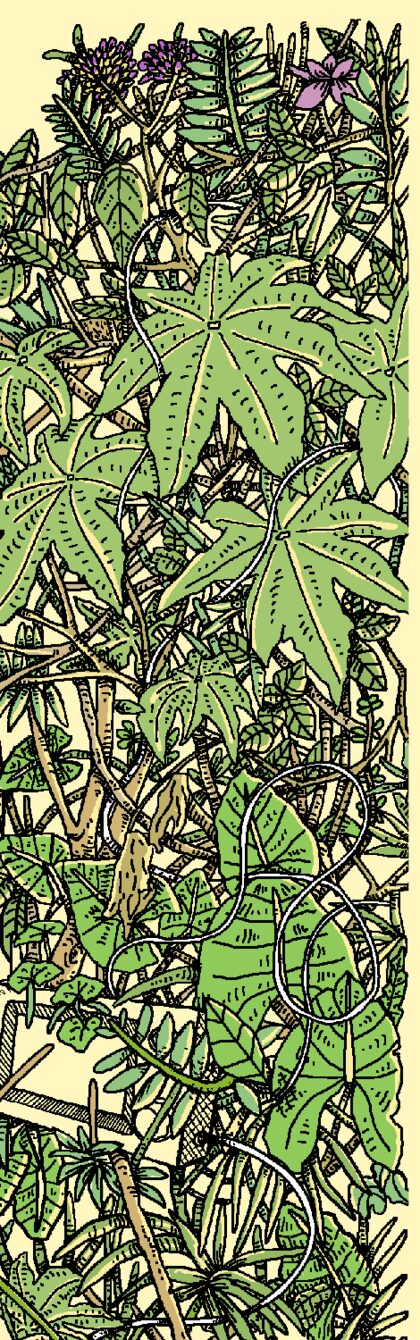
\includegraphics[height=\paperheight]{img/foliage-strip.jpg}};
    \node[anchor=north west,inner sep=0] at ($(current page.north west)+(1.0cm,-1.0cm)$)
      {
\includegraphics[height=2.2cm]{img/hermes-logo.png}};
    \node[anchor=north west,text width=8.6cm,inner sep=0] at ($(current page.north west)+(1.0cm,-4.0cm)$) {%
      {\fontsize{30}{32}\selectfont\bfseries THANK YOU}\par\vspace{0.25em}
      {\color{horange}\rule{3.5cm}{2.5pt}}\par\vspace{0.8em}
      \small
      \faGithub\ \ github.com/Rhizomatica/mercury\par\vspace{0.3em}
      \faGlobe\ \ hermes.radio\par\vspace{0.3em}
      \faBook\ \ docs/ in the repository: modes, carousel, specs, channel model\par\vspace{1.0em}
      {\scriptsize\color{hdkmauve}Mercury is free software (GPL-3.0-or-later).\\ This presentation: CC BY-SA 4.0.}};
  \end{tikzpicture}
\end{frame}

\end{document}
